\documentclass[sigconf,review]{acmart}
\setcopyright{none}

\begin{document}
\title{Bluesky and the AT Protocol: Usable Decentralized Social Media}
\author{Martin Kleppmann}
\email{martin@kleppmann.com}
\orcid{0000-0001-7252-6958}
\affiliation{%
  \institution{TU Munich}
  \city{Munich}
  \country{Germany}
}

\author{TODO: review author list}
\author{Paul Frazee, Jake Gold, Jay Graber}
\author{Daniel Holmgren, Devin Ivy, Jeromy Johnson}
\author{Bryan Newbold, Jaz Volpert}
\affiliation{%
  \institution{Bluesky PBC}
  \country{United States}
}

\begin{abstract}
TODO
% an architecture inspired by the web itself, but modernized to include streams of real-time updates and cryptographic authentication.
\end{abstract}

\begin{CCSXML}
<ccs2012>
   <concept>
       <concept_id>10002951.10003260.10003282.10003292</concept_id>
       <concept_desc>Information systems~Social networks</concept_desc>
       <concept_significance>500</concept_significance>
   </concept>
   <concept>
       <concept_id>10003033.10003106.10003114.10003118</concept_id>
       <concept_desc>Networks~Social media networks</concept_desc>
       <concept_significance>500</concept_significance>
   </concept>
   <concept>
       <concept_id>10003456.10003457.10003490.10003507.10003508</concept_id>
       <concept_desc>Social and professional topics~Centralization / decentralization</concept_desc>
       <concept_significance>300</concept_significance>
   </concept>
 </ccs2012>
\end{CCSXML}

\ccsdesc[500]{Information systems~Social networks}
\ccsdesc[500]{Networks~Social media networks}
\ccsdesc[300]{Social and professional topics~Centralization / decentralization}

\keywords{social media, decentralization, federation, web architecture}
\maketitle

\section{Introduction}

Over the last two decades, social media services have evolved from a fun curiosity into a cornerstone of civic life~\cite{Barabas:2017}.
This development has been accompanied by increasing unease that mainstream ``digital town squares'', such as Twitter/X or Facebook, are under the control of a single corporation, and may change their policies on the whim of their leaders~\cite{Yeung:2023}.
Their operations are opaque (e.g.\ regarding which content is recommended to users), and their users lack agency over their user experience.
As a result, there has been increasing interest in decentralized social networks, of which the \emph{fediverse} around the ActivityPub protocol~\cite{ActivityPub} and the Mastodon software~\cite{Mastodon} is perhaps the best known (we review a selection of decentralized social networks in Section~\ref{sec:related-work}).

However, decentralization also introduces new challenges.
For example, in the case of Mastodon, a user needs to choose a server when creating an account.
This choice is significant because the server name becomes part of the username; migrating to another server implies changing username, and preserving one's followers during such a migration requires the cooperation of the old server.
If a server is shut down without warning, accounts on that server cannot be recovered~-- a particular risk with volunteer-run servers.
In principle, a user can host their own server, but only a small fraction of social media users have both the technical skills and the inclination to do so.

The distinction between servers in Mastodon introduces complexity for users that does not exist in centralized services.
For example, a user viewing a thread of replies in the web interface of one server may see a different set of replies compared to viewing the same thread on another server, because a server only shows those replies that it knows about~\cite{Adida:2022}.
As another example, when viewing the web profile of an account on another server, clicking the ``follow'' button does not simply follow that account; instead, the user needs to enter the hostname of their own server and be redirected to a URL on their home server before they can follow the account.
In our opinion, it is undesirable to burden users with such complexity arising from the federated architecture.

In this paper we introduce the \emph{AT Protocol} (atproto), a decentralized foundation for social networking, and \emph{Bluesky}, a Twitter-style social app built upon it.
A core design goal of atproto and Bluesky is to enable a user experience of the same or better quality as centralized services, while being open and decentralized on a technical level.
We introduce the user-facing features of Bluesky in Section~\ref{sec:product}, and in Section~\ref{sec:architecture} we explain the underlying systems architecture.
The AT Protocol is designed such that for every part of the system there are multiple competing operators providing interoperable services, making it easy to switch from one provider to another.

Decentralization alone is not able to solve some of the thorniest problems of social media, such as misinformation, harassment, and hate speech.
However, by opening up the internals of a service to contributors who are not employees of a particular company, decentralization can enable a marketplace of approaches to these problems.
For example, Bluesky allows anybody to create custom feeds that can apply arbitrary filtering and content selection methods, and custom client software can access all features of the ``official'' app, including moderation tools.
Our hope is that this architectural openness will enable communities to develop their own approaches to managing problematic content, without depending on a centralized service operator to implement these features for them.

For example, researchers wanting to identify disinformation campaigns can easily get access to all content being posted, the social graph, and user profiles on Bluesky.
If they are able construct an algorithm to label suspected disinformation, they can publish their labels in real time for use by other parts of the system, such as custom feed generators or client apps.
One goal of this paper is therefore to bring Bluesky and the AT Protocol to the attention of researchers working on such algorithms, and to invite them to use the rapidly growing dataset of Bluesky content as a basis for their work.

\section{The Bluesky Social App}\label{sec:product}

Bluesky presents itself to users as a straightforward microblogging application in the style of Twitter/X (see Figure~\ref{fig:home-feed}).
The ``official'' client app is available on iOS, Android, and the web; several independently developed client apps are also available, such as Graysky and deck.blue. % TODO: links to those apps
Users can make public posts containing up to 300 characters of text, and up to four images, and they can interact with posts by replying, reposting, or liking.
A user can also follow other users, and the default feed shows posts by accounts that the user is following in reverse chronological order.
There are also alternative feeds that show content on various topics, without the user needing to follow the poster (see Section~\ref{sec:feeds}), which helps users discover each other.

\begin{figure}
    \centering
    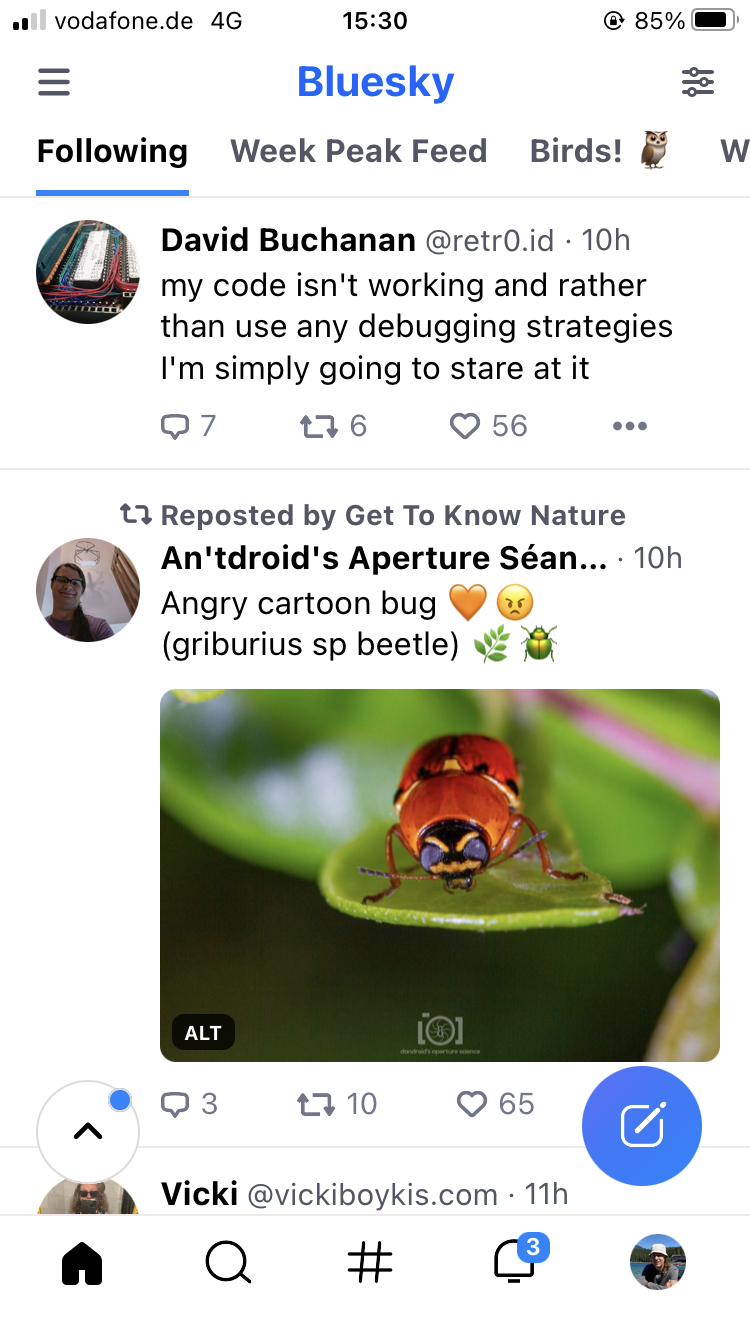
\includegraphics[width=0.7\linewidth]{home-feed.png}
    \Description{A Twitter-like feed of short posts. At the top is a feed selector, in which the default ``Following'' feed is active.}
    \caption{Screenshot of the Bluesky home screen.}
    \label{fig:home-feed}
\end{figure}

\begin{figure}
    \centering
    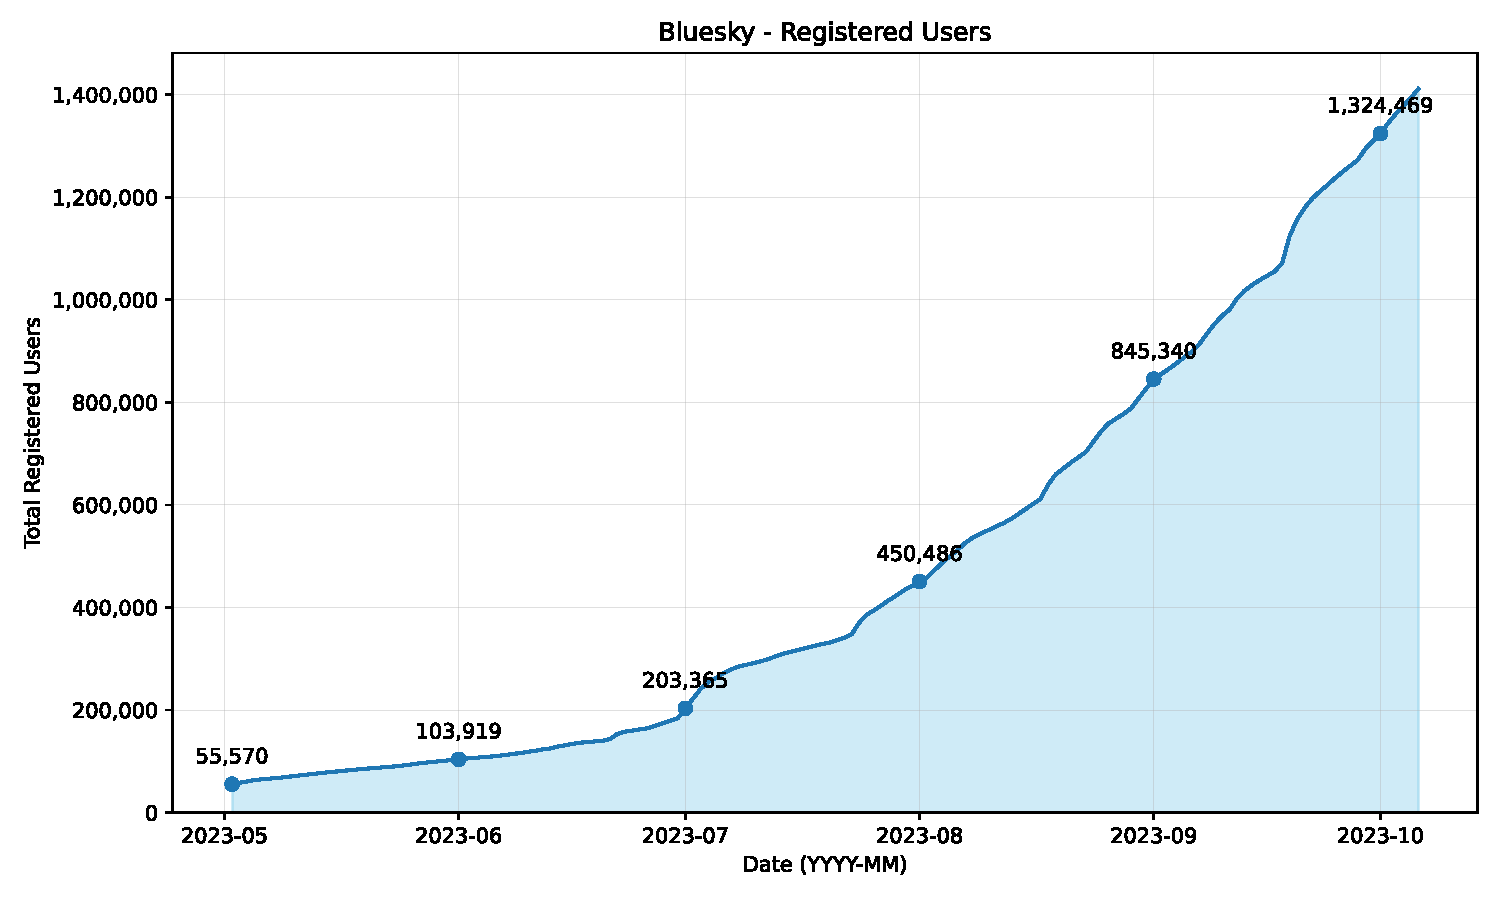
\includegraphics[width=\linewidth]{user-growth.pdf}
    \Description{An exponential growth curve, approximately doubling every month, starting at 55k in May 2023 and exceeding 1.3M in October 2023.}
    \caption{Number of registered Bluesky users from May to October 2023.}
    \label{fig:user-growth}
\end{figure}

Bluesky launched an invite-only beta release in February 2023, and has grown to over 1.5~million registered users in October 2023, as shown in Figure~\ref{fig:user-growth}.
At the time of writing, an invitation code is required to create an account, and codes are available through a waitlist or from an existing user.
Such control over user signups may seem contradictory for a supposedly open and decentralized network, but it has been necessary to limit the load on our infrastructure and to keep abuse at a manageable level.
We intend to remove the need for invite codes in early 2024.

Bluesky, PBC (a public-benefit corporation) develops the official client app and operates the core services; the client and several server-side components are open source under the MIT license~\cite{BlueskyGithub}.
The protocols they use are defined by open specifications~\cite{AtProtoSpecs}.
Several parts of the system, such as feed generators (Section~\ref{sec:feeds}) and various alternative clients~\cite{AtProtoClients} are developed and operated by independent third parties.

\subsection{Moderation Features}\label{sec:moderation}

Bluesky has several moderation mechanisms for managing unwanted content:
\begin{description}
    \item[Content filtering:] Automated systems label potentially problematic content (such as images of a sexual or violent nature, posts promoting hate groups, or spam), and the app's preferences allow users to choose whether to show or hide content in each of these categories in their feeds.
    \item[Mute:] A user can mute specific accounts or threads, which hides the muted content from their own feeds and notifications. The content continues to be visible to other users, and the target does not know that they were muted. A user can also publish a mutelist of accounts, and other users can subscribe to that list, which has the same effect as if they individually muted all of the accounts on the list.
    \item[Block:] One user can block another, which prevents all future interactions (such as mentions, replies, or reposts) between those accounts in addition to muting.
    \item[Takedown:] Users can report content that violates the terms of service to server operators, and the operators can take down violating posts or accounts.
    \item[Custom feeds:] While the aforementioned mechanisms provide negative moderation (helping users avoid content they do not want to see), feed generators (see Section~\ref{sec:feeds}) can actively select high-quality content.
\end{description}

Additional moderation mechanisms are under discussion~\cite{Moderation}.

\subsection{User Handles}\label{sec:handles}

Like on Twitter, a Bluesky user has two names: the \emph{display name} can be almost any string, and the \emph{handle} needs to uniquely identify a user.
A handle, prefixed with an @ sign, is used to mention another user in a post.
Examples can be seen in Figure~\ref{fig:home-feed} (the display name is in bold, and the handle is in a smaller font and lighter color).

The need for handles to be unique creates challenges in decentralized systems, since it requires an authority that determines which handle is assigned to which user.
Mastodon's approach is to include the server name in the handle, which makes it difficult to move to another server.
An alternative would be to use a blockchain-based naming system, such as the Ethereum Name System (ENS)~\cite{ENS}; this has the disadvantage of requiring the user to buy cryptocurrency in order to create an account, which we wanted to avoid.

Instead, Bluesky and atproto use DNS domain names as handles.
If a user already owns a domain name, they can claim it as their Bluesky handle by adding a DNS record or by hosting a file under a \texttt{.well-known} HTTPS URL on that domain~\cite{DomainHandle}.
Users can also buy a new domain name within Bluesky, via a partnership with a domain registrar~\cite{PurchaseDomain}.
Alternatively, users can sign up for a subdomain of \texttt{.bsky.social} for free.

Using DNS domain names as handles has several advantages:
\begin{itemize}
    \item We leverage the existing infrastructure of ICANN, registrars, and name servers, including for example the dispute resolution procedures for trademarks.
    \item Domain names are a well-known concept even among non-technical users, and they are short and simple.
    \item A user can move to a different server without changing their handle.
    \item Users do not need to host their own server to use their own domain name; a DNS record requires only a one-time setup and no ongoing maintenance.
    \item For organizations and people that already have a well-known domain name, using that name makes it easy for users to check that their Bluesky account is genuine. For example, the New York Times' handle is \texttt{@nytimes.com}.
    \item An organization can easily allow their staff to demonstrate their affiliation by granting them handles that are subdomains of the organization's main domain name (comparable to institutional email addresses). For example, a journalist's handle may indicate that they are at a particular news organization.
    \item Providers wanting to offer free subdomains can do so at very little cost.
\end{itemize}

\subsection{Custom Feeds and Algorithmic Choice}\label{sec:feeds}

Several decentralized social networks choose to offer only a reverse-chronological feed of posts from accounts the user is following~-- a backlash against the opaque content recommendation algorithms employed by mainstream centralized social networks.
For example, Mastodon advertises itself as having ``no algorithms or ads to waste your time''~\cite{Mastodon}.

Our belief is that the problem lies not with algorithms \emph{per se}, but rather with centrally controlled, opaque algorithms that remove user agency and prioritize user engagement over all else, e.g.\ by promoting controversial posts.
Good recommendation algorithms can help users discover content that is relevant to them and find new accounts to follow~-- especially important for new users who are not yet following many accounts.
They are also helpful for surfacing content on a particular topic, whereas following a user means seeing all of their posts, which might be on a mixture of topics, not all necessarily interesting to all followers.

Bluesky, PBC offers a selection of feed generation algorithms of its own, and also allows anybody to create their own feed generator~\cite{CustomFeeds}.
The goal is to offer an open and diverse ``marketplace of algorithms'' in which communities can adapt the system to suit their needs, and users have more agency over how they spend their time and attention~\cite{AlgorithmicChoice}.
TODO: how many custom feeds have been created to date? link to section about how feed generators work.

In Figure~\ref{fig:home-feed}, a selection of bookmarked feeds is given at the top of the screen; in this example, the selected ``Following'' feed is the default reverse-chronological timeline, while ``Week Peak Feed'' (network-wide posts with many likes from the last week) and ``Birds!'' (photos and posts from birdwatchers) are third-party feeds.
A feed generator can use arbitrary criteria to select its content.
For example, the birdwatching feed uses manual review of accounts in combination with a \#birds hashtag or a feather emoji character in posts to identify posts to include.
Alternative approaches, such as machine learning algorithms, are equally possible.

\section{The AT Protocol Architecture}\label{sec:architecture}

Almost all data created by Bluesky users is public; in particular, this includes user profiles, posts, follows, and likes.
Blocking actions are also public; however, we are investigating mechanisms for making blocking information private~\cite{PrivateBlocks}.
At present, Bluesky does not support direct messages, which would need to be private.
Only a small amount of user state is currently private: any muted accounts and threads, and the unread status of notifications.

% Labeling services https://github.com/bluesky-social/proposals/tree/main/0002-labeling-and-moderation-controls

% Federation architecture https://blueskyweb.xyz/blog/5-5-2023-federation-architecture

\section{Related Work}\label{sec:related-work}

% https://activitypub.rocks/

% https://scuttlebutt.nz/
% https://github.com/lens-protocol/core
% https://nostr.com/
% "the Nostr protocol powers Minds and Snort, among other decentralized social media"

% https://www.farcaster.xyz/
% https://github.com/farcasterxyz/protocol/blob/main/docs/OVERVIEW.md
% https://www.varunsrinivasan.com/2022/01/11/sufficient-decentralization-for-social-networks

% for likes, the record is around 100 bytes, and the the MST tree stuff is anywhere from 1-4kb (depending on the repo and other randomness in the MST), usually averaging around 2.5Kb.
% https://github.com/bluesky-social/discuss/discussions/16#discussioncomment-7233086

\begin{acks}
TODO
\end{acks}

\bibliographystyle{ACM-Reference-Format}
\bibliography{references}
\end{document}
